\chapter{Navrhování algoritmů}

\section{Časová a prostorová složitost algoritmů}
	Abychom mohli porovnávat algoritmy, řešící stejný problém, mezi sebou a rozhodnout se kdy který algoritmus použít, slouží nám k tomuto účelu základní dvě míry pro porovnání.
\begin{itemize}
	\item časová složitost
	\item prostorová složitost
\end{itemize}
	Časová složitost vyjadřuje jak dlouho bude výpočet podle daného algoritmu trvat, obdobně prostorová složitost nám vyjadřuje kolik prostoru, tedy paměti, danému algoritmu budeme muset poskytnout pro výpočet. Je očividné že vyjadřovat časovou složitost v sekundách a prostorovou v bytech by vzhledem k různému hardwaru, či různé implementaci nebylo příliš vhodné. Pro popis složitosti algoritmu tedy zavádíme pojem \textit{Asymptotická složitost}.
	
\subsection{Asymptotická složitost}
	Asymptotická složitost se vyjadřuje jako matematická funkce, popisující závislost využití paměťového prostoru nebo výpočetního výkonu na velikosti vstupních dat $N$. Důležité je že tato funkce je neklesající a vyjadřujeme ji pouze jako třídu složitosti, tedy typ funkce a ne jako přesné vyjádření. Pro příklad funkce $\mathcal{O} (1000N^2) $ nebo $\mathcal{O} (N^2 + 1000N)$ jsou třídy složitosti $\mathcal{O} (N^2)$. Tedy zanedbáváme multiplikativní konstantu, aditivní konstantu a nižší řády funkce, protože nás zajíma jak se bude měnit časová náročnost s velikostí vstupních dat.
	Tím že zanedbáváme multiplikativní, aditivní konstantu a nižší řády funkce, může se vyskytnout případ kdy algoritmus s horší asymptotickou časovou složitostí proběhne rychleji než algoritmus s lepší asymptotickou časovou složitostí. Máme ovšem jistotu že existuje vstup o velikosti $N_0$, kde toto přestane platit. Při praktickém použití toto může nastat v případě, kdy asymptoticky rychlejší algoritmus má složitější implementaci a prostředky vynaložené na režiji převyšují výhody algoritmu. [něco citovat]
	
\begin{figure}[h]
  \centering
  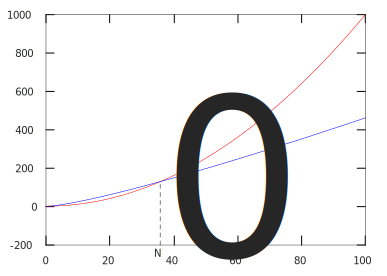
\includegraphics[width=7.5cm]{./pictures/3/time_complexity.pdf}
  \caption{Graf znázorňující průběh algoritmu v závislosti na $N$}
  \label{fig:3-time_complexity}
\end{figure}
	
	
	 Pro vyjádření časové složitosti můžeme využít různé varianty.
\begin{itemize}
	\item Horní odhad složitosti - $\mathcal{O} (f(N))$
	\item Průměrná složitost - $\Theta (f(N))$
	\item Dolní odhad složitosti - $\Omega (f(N))$
\end{itemize}	
	Nejčastěji využívaný odhad je takzvaná \textit{Omikron notace}, která vyjadřuje horní odhad, tedy nejhorší možný případ jakým se může algoritmus chovat. V tomto případě máme jistotu že algoritmus bude asymptoticky probíhat stejně rychle nebo rychleji v případě časové složitosti. V některých případech se vyplatí uvádět i průměrnou složitost, tedy složitost, která nastává při nějakém náhodném rozložení vstupních dat. Tato situace pak lépe vystihuje praktické použití algoritmu, ale nemáme jistotu že se bude chovat asymptoticky hůře. Poslední variantou je dolní odhad složitosti, který nám naopak vyjadřuje že algoritmus se bude chovat stejně nebo hůře než je uvedeno.
	
\subsection{Stanovení časové složitosti}
	Časovou složitost algoritmu můžeme stanovit matematickou analýzou nebo empiricky. U jednoduchých algoritmů většinou není problém stanovit složitost
	
	
	
	
\section{Metody návrhů algoritmů}

\subsection{Metoda hrubé síly}
	Patří k nejjednodušším metodám algoritmizace. Jak vyplývá z názvu, v této metodě budeme postupovat hrubou silou, tedy v praxi to znamená že algoritmus bude zkoušet všechny možné kombinace řešení, než dosáhne výsledku. Mezi výhody patří jednoduchá implementace a snadné porozumění algoritmu. Tyto algoritmy lze využívat pouze pro malé vstupní množiny díky jeho asymptotické složitosti. V praxi lze algoritmy využít i jako doplněk složitějších algoritmů, kde by režije, jako je volání funkcí nebo vytváření objektů, zabralo více času než na tuto malou množinu použít algoritmus hrubé síly.
	
